\documentclass[a4paper,12pt]{report}
\usepackage{styles/report_format}
\usepackage[style=ieee]{biblatex}
\addbibresource{references.bib}
	
\renewcommand{\labelenumi}{(\roman{enumi})}



\usepackage{amsmath, amsthm, amssymb}
 % Some extra symbols
\usepackage[bottom]{footmisc}
%\usepackage{cite}
\usepackage{graphicx}
\usepackage{longtable}
\usepackage{algorithm}
\usepackage{algorithmic}




% Directory of figures
\graphicspath{{figures/}}

% Times New Roman, Requires XeLaTeX or LuaLaTeX
\RequirePackage{fix-cm}
\usepackage{fontspec}
\setmainfont{Times New Roman}


% Numbering at bottom
\usepackage{fancyhdr}
\pagestyle{fancy}
\fancyhf{}% Clear page header/footer
\renewcommand{\headrulewidth}{0pt}% No header rule
\fancyfoot[C]{\thepage}

% Page Margins
\usepackage[top=3.5cm,bottom=2cm,left=3.5cm,right=2cm]{geometry}

% Prevent hypanated words
%\hyphenpenalty=100000

% COVER PAGE parameters
\title{AUTOMATIC MUSIC TRANSCRIPTION}
\turkcebaslik{TITLE OF THE PROJECT}
\author{Name Surname}
\subyear{2021}

% APPROVED BY PAGE parameters
\supervisor{Assist. Prof. Dr. Dionysis Goularas}
\examineri{Assist. Prof. Dr. Esin Onbaşıoğlu}
\examinerii{Prof. Dr. Sezer Gören Uğurdağ}
\dateofapproval{.../.../2021}

\begin{document}
\pagenumbering{roman}

% COVER PAGE

\makecoverpage
    
% BLANK PAGE
\clearpage\mbox{}
\clearpage    
\addtocounter{page}{-1}
    
% APPROVAL PAGE
\makeapprovalpage

% ACKNOWLEDGEMENTS PAGE
\begin{acknowledgements}
First of all I would like to thank my advisor ... 
for his guidance and support throughout my project.

Also I would like to thank my parents for their support and encouragement throughout my education up to the present.
\end{acknowledgements}

% ABSTRACT PAGE
\begin{abstract}
Automatic music transcription is an ongoing research field as a branch of music information retrieval and digital signal processing.  It can be used for transcribing high amounts of music at once or categorizing and indexing music on databases for pattern matching or machine learning. It can be a challenge to create a general purpose algorithm as pitch is a concept related to human perception and harder for complex signals of polyphonic music. This project focuses on monophonic music only, by explaining several existing approaches and demonstrating the implementation of one of them.
\end{abstract}

% ÖZET PAGE
\begin{ozet}
Otomatik müzik transkripsiyonu onyıllardır sürmekte olan bir araştırma alanıdır. Müzikten bilgi edinme ve dijital sinyal işlemenin bir alt dalıdır. Bir seferde çok sayıda transkripsiyon yapma, veri tabanları üzerinde kategorizasyon ve indeksleme ile makine öğrenmesi için kullanılabilir. Duyulan bir nota insan kulağıyla ilgili bir durum olduğu için belirlenmesini sağlayacak kesin bir algoritma ortaya konulması sorunludur. Karmaşık polifonik sesler için daha sorunludur. Bu raporda, var olan birkaç yöntemden söz edilmekte ve içlerinden birinin uygulanışı gösterilmektedir.
\end{ozet}

% TABKE OF CONTENTS
\tableofcontents

% LIST OF FIGURES
\listoffigures

%LIST OF TABLES
\listoftables

% ABBREVIATIONS
\begin{symbols-abbreviations}
\sym{$\delta_t$}{Threshold}
\sym{$f_0$}{Fundamental frequency}
\sym{$\circ$}{Hadamard Product}
\sym{$\mu$}{Magnitude}
\sym{ReLU}{Rectifier Function}
\sym{$\rho$}{Resampling Function}
\sym{S}{Spectrogram}
\sym{$\hat{S}$} {HPS Applied Spectrogram}
\sym{$\varphi$}{Phase}
\sym{X} {Complex STFT Output}
\sym{}{}
\sym{ABI}{Application Binary Interface}
\sym{CLI}{Command Line Interface}
\sym{CPU}{Central Processing Unit}
\sym{DFT}{Discrete Fourier transform}
\sym{DSP}{Digital Signal Processing}
\sym{FFT}{Fast Fourier Transform}
\sym{FFI}{Foreign Function Interface}
\sym{GPU}{Graphics Processing Unit}
\sym{MIDI}{Musical Instrument Digital Interface}
\sym{MIR}{Music Information Retrieval}
\sym{PDA}{Pitch Detection Algorithm}
\sym{STFT}{Short Time Fourier Transform}
\sym{VRAM}{Video Ram (Random Access Memory)}
\sym{WAV}{Waveform Audio File Format}


\end{symbols-abbreviations}

% CONTENT
\chapter{INTRODUCTION}
\label{chapter:introduction}
\pagenumbering{arabic}

\section{Automatic Music Transcription}
In music, transcription is notating a piece or a melody and documenting it on a sheet with a format which can later be read by a musician and reproduced as sound. Notating a piece is generally done by a musician by listening it played and writing down the notes with their durations and the speed which it should be played. Transcription may also include an arrangement of the original piece to fit one or more different instruments and musical styles. The end product of this process is called \textit{sheet music} (Figure \ref{fig:sheetmusic}). It can be said that, transcription is a form of recording.
\vskip\baselineskip
\begin{figure}[htbp]
\begin{center}
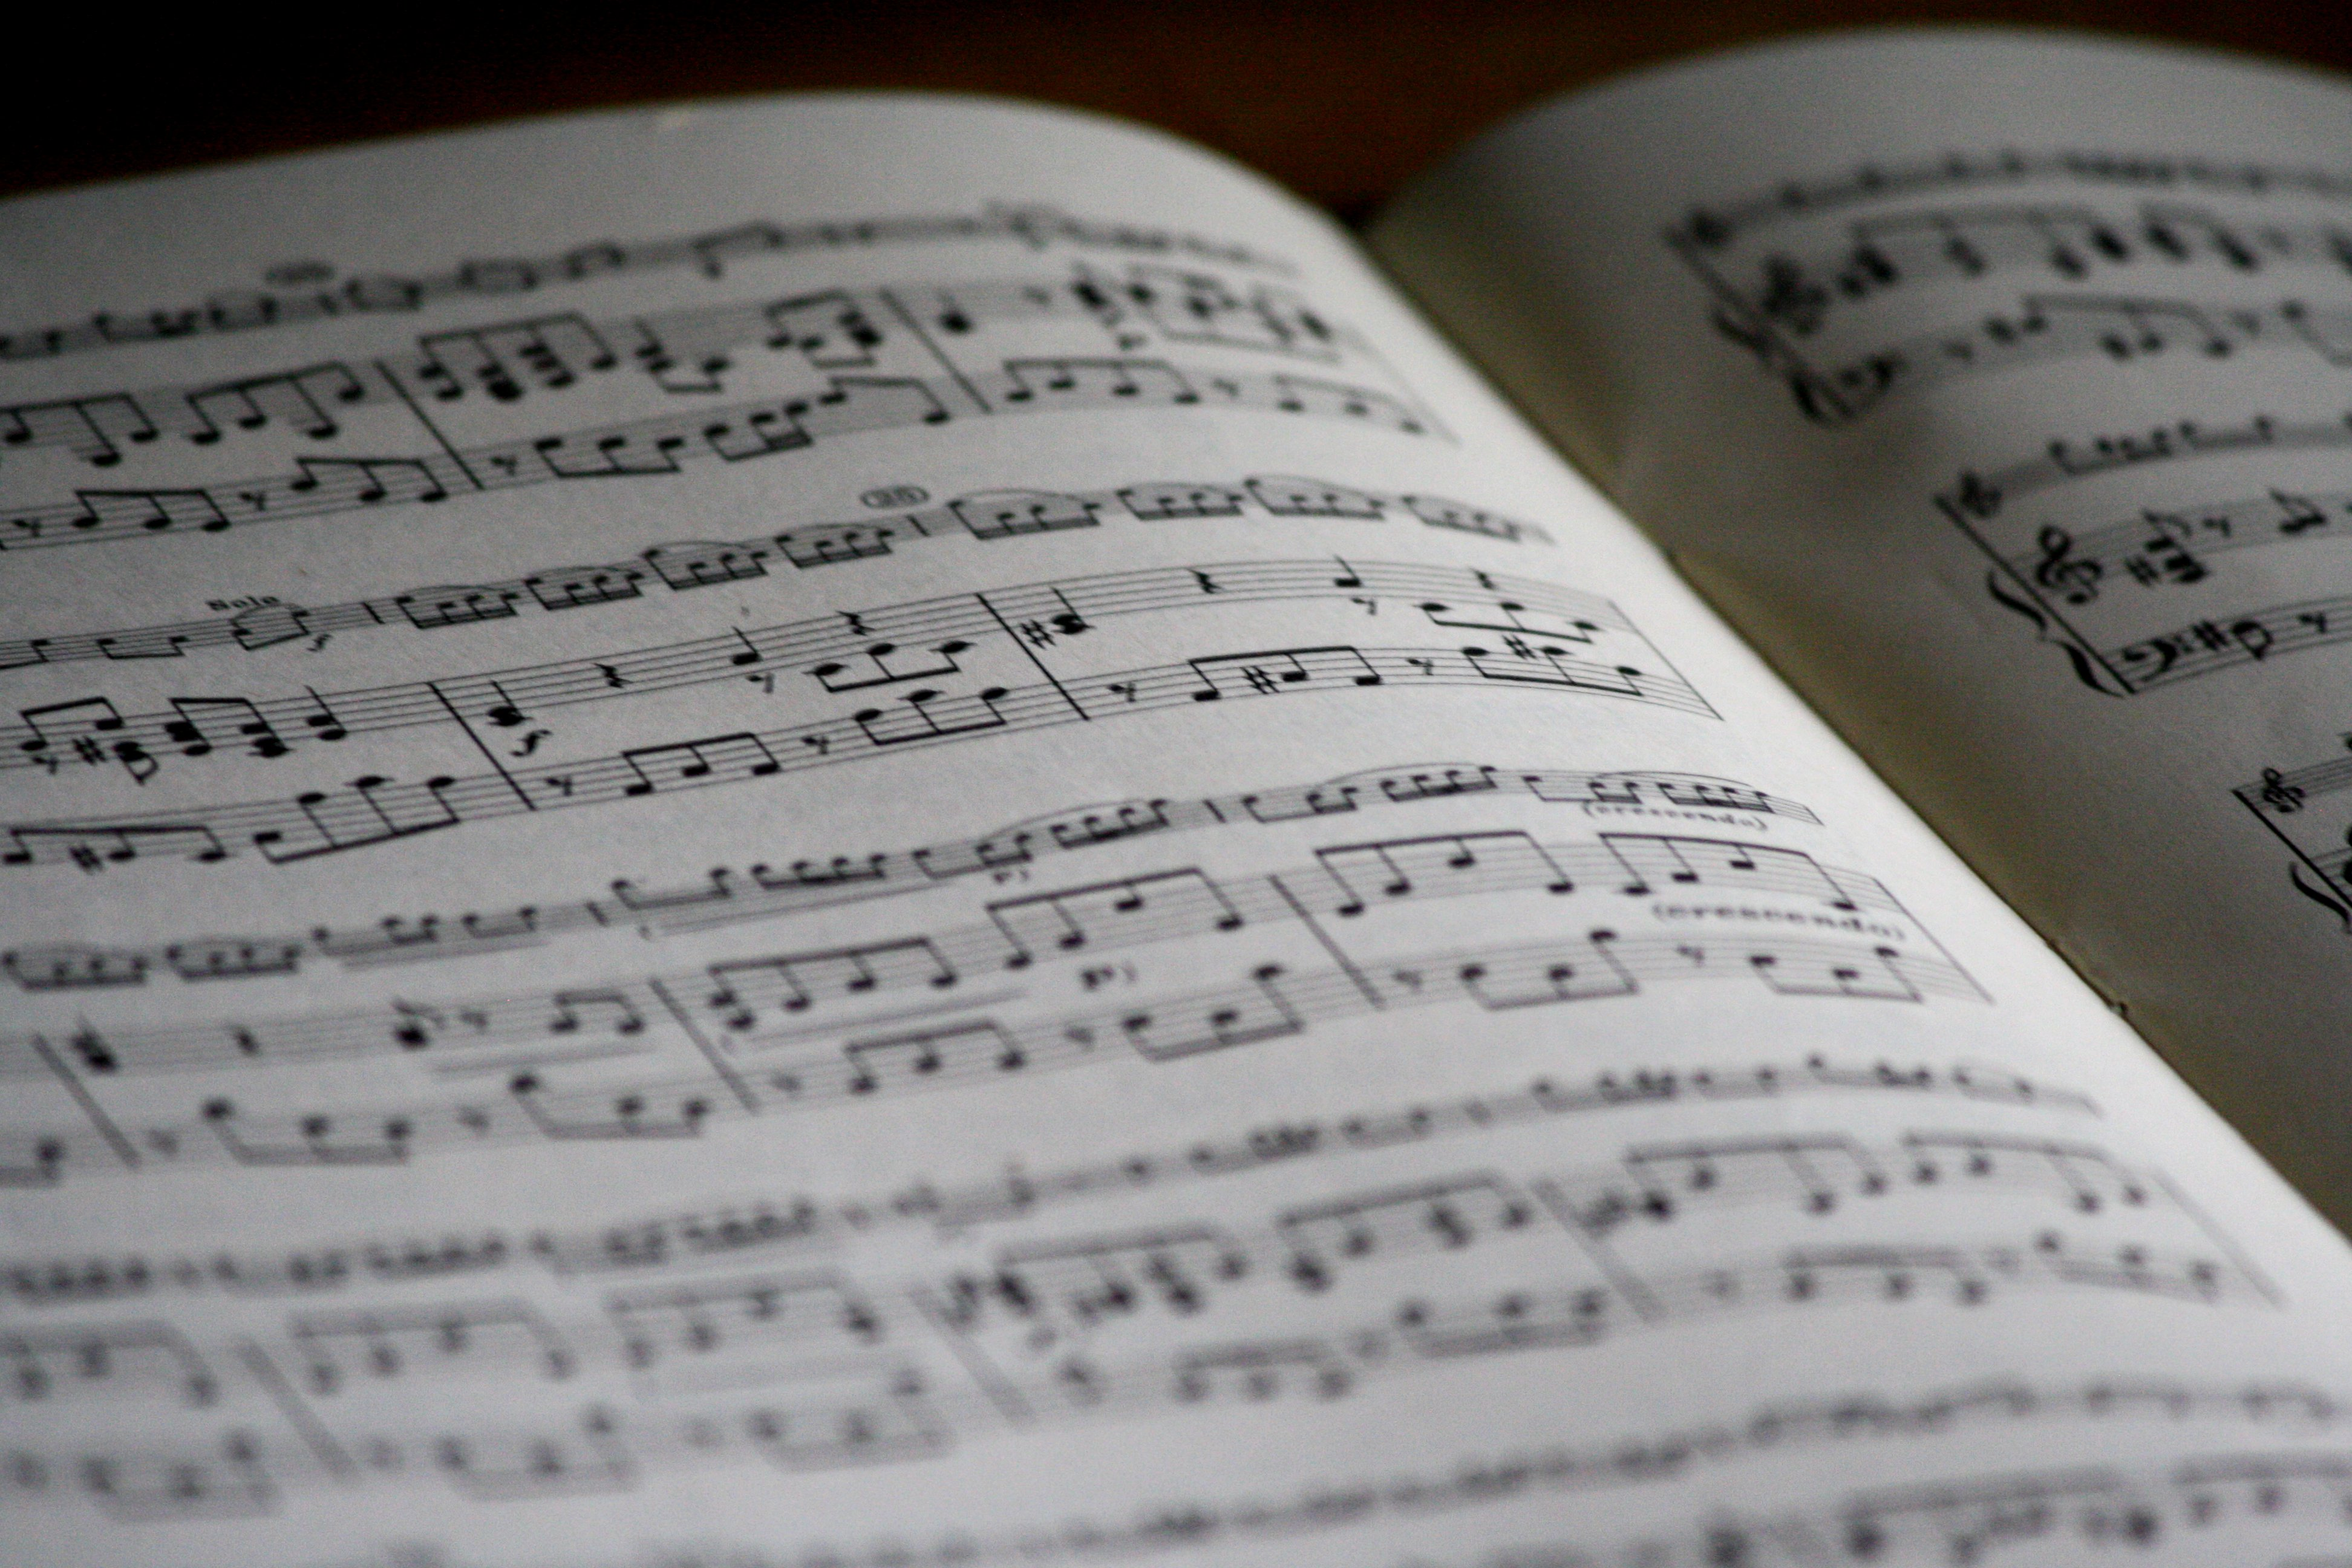
\includegraphics[scale=0.1,keepaspectratio]{sheet.jpg}
\end{center}
\caption{Sheet Music}
\vskip\baselineskip % Leave a vertical skip below the figure
\label{fig:sheetmusic}
\end{figure}

In that sense a MIDI file can be considered a digital sheet music as it can be used to reproduce a melody by keeping information about notes and timings. MIDI files can be inserted into appropriate software where the music it represents can be heard audibly or simply displayed as a conventional visual sheet music. This makes MIDI a convenient format for the digital age.

\textit{Automatic music transcription} is automating the aforementioned process by detecting pitches, patterns and melodies by putting the signal through dedicated hardware or software on general purpose computers which takes the musical audio as an input and outputs the notes in some format. Although it may be frowned upon by some musicians and manually doing transcriptions is a valuable exercise for musicianship, automation in this field have several benefits which are discussed in Section \ref{motivation}. Automatic music transcription at its core involves identifying the pitches and onsets, then mapping this information into traditional music notation. 

Automatically transcribing music is contained within the field of Digital Signal Processing (DSP), alongside of various other signal processing and analysis methods. There are also many similarities and common parts between this technique and speech recognition but this in not in the scope of this project.

\subsection{Pitch Detection}
Pitch detection is the detection of individual notes which often together make up a melody by analysing a signal. It should be noted that a single frequency does not necessarily correspond to a pitch and it often does not. What is heard from an instrument as pitch is usually a composite of harmonics or partials. There is no single perfect Pitch Detection Algorithm that works for all cases, therefore there are a several methods \cite{paper:5} for pitch detection. A typical PDA does estimation on quasi-periodic signals to get a frequency value.  

\textit{Zero crossing} is the simplest of these methods. It works by getting the frequency through counting the points where the sinusoidal audio signal's value changes sign. Although simple and fast, it fails where a moderately complex waveform consisting of more than a single frequency or noise may be present.

\textit{Autocorralation} \cite{paper:3} uses the fact that a periodic signal will be similar from one period to the next. It works by correlating the signal with a shifted version of itself. As the shift value reaches the fundamental period i.e. the fundamental frequency, difference between the shifted and the original signals decrease. Period is revealed as the autocorrelation function approaches zero for a given shift.

%\subsubsection{Frequency Domain Methods}
Both zero crossing and autocorrelation are methods working on the time domain. There also exists methods that work on the frequency domain such as:

\textit{Harmonic product spectrum} which works by compressing the spectrogram along the frequency axis some number of times, aligning the starting positions and multiplying all the resulting compressed spectrograms. This makes the fundamental frequencies become more distinguishable with higher magnitudes than the rest. This process is explained more in depth in Section \ref{hps}

\textit{Cepstrum Analysis} \cite{paper:4} is a form of spectral analysis where the output is the Fourier transform of the log of the magnitude spectrum of the input waveform. This methods is usually used for speech signals with many and evenly spaced partials. 

\textit{Maximum Likelihood Estimation} \cite{paper:4, paper:5} is a statistical method. It involves computing probabilities for a set of candidate fundamental frequencies and finding the maximum that fits the observed data of partials of the pitch. 

\subsection{Beat Detection}
Beat detection is the detection of a repeated time interval between perceived pulses of a melody. A BPM (Beats Per Minute) value determines the intended speed of the composition. A beat is mostly relevant to percussion instruments.

Since notes usually start on a beat, integrating a beat detection algorithm into transcription is potentially beneficial to the accuracy.

\section{Terms}
\begin{itemize}  
\item \textit{Pitch} is a perceptual property of sound which makes it possible to judge sounds as "higher" and "lower" in the sense associated with musical melodies. Pitch is irrelevant in the context of inharmonic percussion instruments.
\item \textit{Duration} is an amount of time or a particular time interval: how long or short a note lasts.
\item A \textit{note} is the pitch and duration of a sound, and also its representation in musical notation.
\item A \textit{semitone}, also called a half step or a half tone, is the smallest musical interval commonly used in Western tonal music.
\item \textit{Onset} is the beginning of a musical note.
\item \textit{Beat} is the basic unit of time, the pulse of the melody which a listener can tap their foot.
\item What is perceived as pitch from an audio source such as an instrument or singer often consist of a fundamental frequency and its overtone partials which reside at integer multiples of the fundamental unless it is an inharmonic instrument. These overtones are called \textit{harmonics}. Harmonics look like a comb (Figure \ref{fig:comb}) on a spectrogram with decreasing amplitudes as the frequency gets higher. By analysing the characteristics and distribution of these harmonics a fundamental can be determined.
\vskip\baselineskip
\begin{figure}[htbp]
\begin{center}
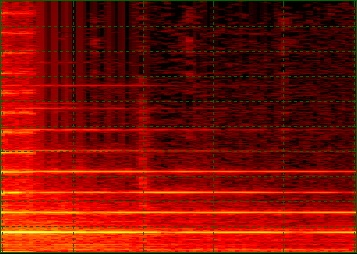
\includegraphics{comb.jpg}
\end{center}
\caption{Harmonic Spectrum on the Spectrogram}
\vskip\baselineskip % Leave a vertical skip below the figure
\label{fig:comb}
\end{figure}
\item \textit{Fundamental Frequency} is the lowest frequency of a periodic waveform. In music, the fundamental is the musical pitch of a note that is perceived as the lowest partial present abbreviated as $f_0$. In terms of Fourier series the fundamental frequency is the lowest frequency sinusoidal in the sum. 
\item \textit{Timbre} is the perceived sound quality which makes it possible to distinguish different sources of same pitch such as different types of instruments. Timbre of an instrument comes from the different combinations of the partials magnitudes.
\item In music, \textit{monophony} is the property of a melody that is created by a single instrument or singer and without the use of any chords, a single note at a time. On the other hand a \textit{polyphonic} melody involves chords and/or multiple instruments or singers simultaneously.
\item In signal processing \textit{sampling} is a way to represent a continuous time signal with discrete values and \textit{sampling rate} is how many discrete values there are in a second of digital signal in other words, samples per second.
\item A \textit{spectrogram} is a way to visually represent the frequency spectrum's change against time of a signal. It is generally showed as two axes for time and frequency and a third dimension for the amplitudes of particular frequencies. Example figures can be seen in Section \ref{design-and-implementation}
\item \textit{Fourier transform} or Fast Fourier Transform (FFT) is an algorithm that gets the components from a signal that is the sum of multiple sinusoids (Figure \ref{fig:fourier}). For a finite sequence of equally-spaced samples such as digital recordings, FFT calculates the Discrete Fourier Transform (DFT).
\vskip\baselineskip
\begin{figure}[htbp]
\begin{center}
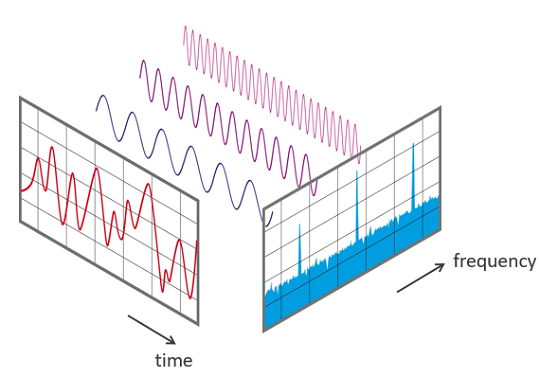
\includegraphics[scale=0.9]{fft.png}
\end{center}
\caption{Fast Fourier Transform}
\vskip\baselineskip % Leave a vertical skip below the figure
\label{fig:fourier}
\end{figure}
\item \textit{Short-Time Fourier Transform} (STFT) is used to get the frequency spectrum that is changing over time by dividing the signal into segments and applying FFT on each. 
\item When a segment of a signal is multiplied with a \textit{Windowing Function} its shape changes
\item \textit{MIDI} is a communication protocol for digital interfaces which carries event messages such as pitch, velocity and others. 
\end{itemize}

\section{Motivation}
\label{motivation}
\subsection{Accessibility}
Musicians who may not have sufficient transcription skills or simply does not have the time to do so, dealing with excess number of transcription jobs may find an automatic transcription software useful.  
\subsection{As a Basis for Other Applications}
Automatic Music Transcription is a form of Music Information Retrieval (MIR). MIR techniques are used in various fields. Retrieved information can be used for creating databases to categorize music with indexing and pattern matching or training machine learning algorithms and music generation. Also, it can be said that converting an audio file into MIDI is a form of compression.

\section{Scope and Limitations}
\begin{itemize}
\item One of the common problems of pitch detection algorithms \cite{paper:4} is the octave problem where an upper harmonic is mistaken for the fundamental if the actual fundamental has low power. 
\item Pitch detection is a term that is relevant to human hearing and involves pseudo acoustics, therefore difficult to implement as a definite algorithm.
\item In terms of automatic transcription, writing down the detected notes and timings to fit a notation is a challenge also with different techniques involving different instruments. For example natural harmonics.
\item Polyphonic pitch detection is problematic because of the many harmonics of different pitches at a time being in the same spectrum.
\end{itemize} 

\section{Problem Definition}

\section{Requirements}

\chapter{BACKGROUND}
\label{chapter:background}
\section{Previous works}
Automatic music transcription has been an ongoing research for decades. First use of the term  is by audio researchers James A. Moorer, Martin Piszczalski, and Bernard Galler in 1977. They believed that a computer program can exist that analyses a digital recording and detect melody lines and chord patterns \cite{paper:6}. Piszczalski and Galler's work was focused on single instruments with strong fundamentals utilising FFT. 

Moorer \cite{paper:7} was the first in the literature to attempt separation of simultaneous sounds with some constraints. 

Extensive research was done by a group at Stanford’s CCRMA \cite{paper:8} in polyphonic pitch-analysis
during the early 1980s which gave way to build polyphonic pitch-tracking systems, largely for acoustic piano.  

Similar works continued \cite{paper:6} by Vercoe and Cumming in 1988, R. C. Maher in 1990, Kashino and Tanaka in 1992, Hawley in 1993, Martin in 1996, Vercoe, Gardner and Scheirer in 1998 where new techniques and/or improvements are introduced by each.

\chapter{ANALYSIS}
The complete process can be seen on Figure \ref{fig:activity}
\section{Filtering}
First, a high pass filter with a chosen cut off frequency is applied to the digital signal
using discrete convolution (Equation \ref{eq:conv}) This process eliminates low
frequencies which we might not be interested in and provides noise reduction.
\begin{equation}
\label{eq:conv}
(f*g)[n] = \displaystyle\sum_{m=-\infty}^{\infty} f[m]g[n-m]
\end{equation}

\section{Spectrograms}
Then, from the resulting filtered samples two separate spectrograms are calculated, one with relatively large and another with  relatively small window size later to be combined. The need for two separate spectrograms and the combination technique is explained in Section \ref{combined}. In discrete-time STFT, input samples are divided into overlapping chunks with a chosen window size and a step size. Applying Fast Fourier Transform on each of these chunks and appending them to a matrix as columns will result in a two dimensional matrix of complex numbers as the STFT output expresses both phase and magnitude. Only the bottom half of the frequency axis is used because of its symmetry. Calculating a spectrogram is done with the following discrete-time short time Fourier transform:
\begin{equation}
X(m,w) = \displaystyle\sum_{n=-\infty}^{\infty} x[n]w[n-m]e^{-jwn}
\end{equation}
where $x$ is the input signal and $w$ is a Gaussian curve window, then getting the magnitudes from the complex values with:
\begin{equation}
S(\tau,w) \equiv |X(\tau,w)|
\end{equation}
where $\tau$ is the time frame and $w$ is the frequency bin. Similarly, $arctan(X(\tau,w))$ gives the phases.

\begin{figure}[htbp]
\begin{center}
\framebox[6.0in]{\begin{minipage}[t]{5.9in}
\begin{algorithmic}
\STATE
\STATE \textbf{Require} audio samples, window size, step size
\STATE $audio\ length \Leftarrow$ number of audio samples
\STATE $spectrogram\ length \Leftarrow (audio\ length-(window\ size-step\ size) )/step\ size$
\STATE $spectrogram\ height \Leftarrow window\ size$
\STATE Form the $spectrogram\ height \times spectrogram\ length$ matrix $\mathbf{X}$
\STATE
\STATE $i \Leftarrow 0, j \Leftarrow 0$
\WHILE{$i < audio\ length - window\ size$}
\STATE $chunk \Leftarrow $ audio samples from index $i$ to $i+window\ size$
\STATE $chunk \Leftarrow chunk \circ (hamming\ function$ of length $window\ size)$
\STATE $new\ column \Leftarrow FFT(chunk)$
\STATE $j^{th}\ column\ of X \Leftarrow new\ column$
\STATE $i \Leftarrow i + step\ size, j \Leftarrow j+1 $
\ENDWHILE
\STATE
\STATE Take rows $0\ to\ (window\ size)/2$ from $X$
\STATE
\end{algorithmic}
\end{minipage}}
\end{center}
\caption[Short Time Fourier Transform Algorithm]{Short Time Fourier Transform Algorithm.}
\label{alg:stft}
\end{figure}
\section{Combined Spectrogram}
\label{combined}
Due to the nature of STFT a resulting spectrogram can either have good frequency resolution or good time resolution depending on the window size. This shortcoming can be mediated by calculating two spectrograms called wideband and narrowband, where wide and narrow refer to the window size used in the STFT and multiplying the corresponding pixel values of the two creating a combined spectrogram \cite{paper:2} which preserves the visual features associated with both. Characteristics of all the spectrograms can be seen in example figures in Section \ref{design-and-implementation}. In practice this can be achieved with the following: 

After getting the two spectrograms $A$ and $B$ such that:
\begin{equation}
A_{m,n} = 
 \begin{pmatrix}
  a_{1,1} & a_{1,2} & \cdots & a_{1,n} \\
  a_{2,1} & a_{2,2} & \cdots & a_{2,n} \\
  \vdots  & \vdots  & \ddots & \vdots  \\
  a_{m,1} & a_{m,2} & \cdots & a_{m,n} 
 \end{pmatrix},
 B_{p,q} = 
 \begin{pmatrix}
  b_{1,1} & b_{1,2} & \cdots & b_{1,q} \\
  b_{2,1} & b_{2,2} & \cdots & b_{2,q} \\
  \vdots  & \vdots  & \ddots & \vdots  \\
  b_{p,1} & b_{p,2} & \cdots & b_{p,q} 
 \end{pmatrix},
 \begin{cases}
 m > p \\
 n < q
 \end{cases}
\end{equation}

they are both resized to match the same shape of height $m$ and length $q$ by calculating the missing values using bilinear interpolation. Then the element-wise multiplication (Hadamard product) takes place like so:
\begin{equation}
C_{m,q} = A_{m,q} \circ B_{m,q}
\end{equation}
where $C$ is the $m \times q$ matrix i.e. the combined spectrogram.

\section{Harmonic Product Spectrum}
\label{hps}

HPS is a process used to make the fundamental frequencies stand out by using the STFT output. This process involves two steps that is repeated as needed. First step is compression with resampling the spectrogram along the frequency axis and second step is multiplying the resulting compressed spectrogram with the original one, element by element by aligning the starting indices. In the first iteration magnitude spectrogram is compressed to half its size, on the next iteration to the third of its size and so on. Compression by an integer makes the partial frequencies of a pitch start to line up on the same frequency as seen on Figure \ref{fig:hps_explain}. The frequency which the partials line up on and make its magnitude higher because of the multiplication is the fundamental ($f_0$). $X(w_n)$  in Figure \ref{fig:hps_explain} are showing the magnitudes of the frequencies in a single time frame. 
\begin{equation}
\hat{S}(\tau,w) = \displaystyle\prod_{r=1}^{R} \rho_r(\tau,w),\hspace{0.2cm} w = \lfloor w_0/R \rfloor
\end{equation}
where $R$ is the HPS rate, meaning that how many times the original (combined spectrogram from Section \ref{combined}) is compressed and $w_0$ is the original spectrograms height. $\rho_r$ is the resampled spectrogram with a new height of $r^{th}$ of the original and calculated as:
\begin{equation}
\label{eq:hps}
\rho_r(\tau,w) = \frac{\displaystyle\sum_{i=0}^{r}S(\tau, rw+i)}{r}
\end{equation}
\newpage
\vskip\baselineskip
\begin{figure}[htbp]
\begin{center}
\framebox[6.0in]{\begin{minipage}[t]{5.9in}
\begin{algorithmic}
\STATE
\STATE \textbf{Require} rate, spectrogram
\STATE Form the $spectrogram.height/rate \times spectrogram.length$ matrix $\mathbf{H}$
\FOR{$r=2$ to $R$}
\STATE $downsampled \Leftarrow$ downsample spectrogram to $r^{th}$ of its size
\STATE $d \Leftarrow$ take rows $0$ to $spectrogram.height/rate$ from downsampled
\STATE $H \Leftarrow H \circ d$
\ENDFOR
\STATE
\end{algorithmic}
\end{minipage}}
\end{center}
\caption[Harmonic Product Spectrum Algorithm]{Harmonic Product Spectrum Algorithm}
\label{alg:hps}
\end{figure}
\vskip\baselineskip
HPS method is fast, inexpensive and reasonably resistant to noise but becuase of the human picth perception being logarithmic it falls short for low frequencies. It is also dependant on the FFT resolution \cite{url:2} that was used for its accuracy. 
\vskip\baselineskip
\begin{figure}[htbp]
\begin{center}
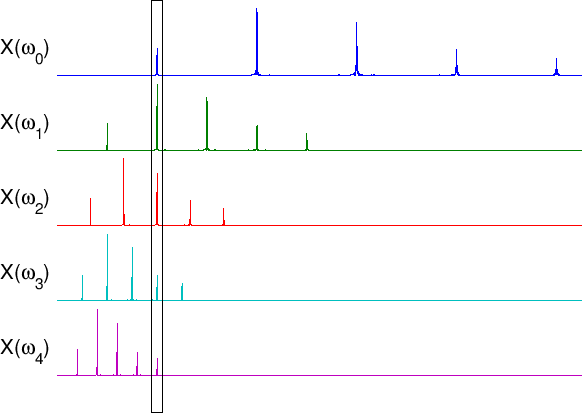
\includegraphics[scale=0.65, keepaspectratio]{hps2.png}
\end{center}
\caption{Harmonic Product Spectrum}
\vskip\baselineskip % Leave a vertical skip below the figure
\label{fig:hps_explain}
\end{figure}

\section{Getting Frequencies}
\label{frequencies}
A fundamental frequency $f_0$ for each time frame is the frequency with the maximum amplitude (Equation \ref{eq:max-freq}) after HPS is applied . 
\begin{equation}
\label{eq:max-freq}
f_0(t) = \max(f_t(x))
\end{equation}

\begin{figure}[htbp]
\begin{center}
\framebox[6.0in]{\begin{minipage}[t]{5.9in}
\begin{algorithmic}
\STATE
\STATE \textbf{Require} spectrogram
\STATE Form an array $F$ with length $spectrogram.length$
\FOR{$i=0$ to $spectrogram.length$}
\STATE F[i] = index of maximum value from spectrogram[i]
\ENDFOR
\STATE
\end{algorithmic}
\end{minipage}}
\end{center}
\caption[Getting Frequencies Algorithm]{Getting Frequencies Algorithm}
\label{alg:freq}
\end{figure}

\subsection{Frequency to Note Conversion}
After a list of frequencies which every value corresponds to a time frame are acquired as seen in Section \ref{frequencies}, this information is combined with the onset detection which is explained in section \ref{onset-detection}. For every note duration which we know the starting and finishing times from the onset detection, a slice from the frequency list corresponding to that time interval is used. This time interval is translated into a single frequency value by taking the mode of the slice and later translated again into a semitone difference using Equation \ref{semitone}

To get the frequency of a note \cite{url:1} on an equal tempered scale following formula is used:
\begin{equation}
\label{eq:fixednote}
f_n = f_a*(\sqrt[12]{2})^n
\end{equation}

where $f_a$ is the known frequency of a fixed note of our choosing. A common choice is $A_4$ which is the A above middle C with a frequency of 440 Hz. n is the number of half steps (semitones) away from the fixed note. A higher note would make $n$ positive and similarly a lower note would make it negative. $f_n$ is the frequency of the note $n$ half steps away from $f_a$

Since we have frequencies and need the notes, Equation \ref{eq:fixednote} has to be reversed as such:
\begin{equation}
\label{semitone}
n = log_{\left(\sqrt[12]{2}\right)} \left(\frac{f_n}{f_a}\right)
\end{equation}

Knowing the $n$ value, we can use it to get the notes' pitches and octaves from a table such as Table \ref{table:sample} or directly calculating.

\begin{table}[thbp]
\vskip\baselineskip 
\caption[Notes' semitone distances to A]{Notes' semitone distances to A.}
\begin{center}
\fontsize{11}{11}\selectfont
\begin{tabular}{|c|c|c|c|c|c|c|c|c|c|c|c|} \hline
-9 & -8 & -7 & -6 & -5 & -4 & -3 & -2 & -1 & 0 & 1 & 2\\ \hline 
$C_4$ & $C_4\sharp/B_4\flat$ & $D_4$ & $D_4\sharp/E_4\flat$ & $E_4$ & $F_4$ & $F_4\sharp/G_4\flat$ & $G_4$ & $G_4\sharp/A_4\flat$ & $A_4$ & $A_4\sharp/B_4\flat$ & $B_4$\\ \hline
\end{tabular}
\label{table:sample}
\end{center}
\end{table}

\section{Onset Detection}
\label{onset-detection}

Onset detection gives the information when a note begins and the last one finishes including rests. It works best with signals where an instrument with high attack and distinct note changes is used. There are energy and phase based approaches for onset detection \cite{paper:1}. For instruments with strong attacks, an increase in energy is expressive and sufficient for onset detection. As for phase, during the steady-state part of a signal most values will be concentrated around zero creating a sharp distribution but on onset points this distribution gets wider and less sharp. Energy approaches fail on the lack of pronounced energy increases and phase approaches are susceptible to phase distortion and to the variations introduced by the phase of noisy components. Combining energy and phase information \cite{paper:1} together a better result can be achieved. 

Two narrowband spectrograms of magnitude and phase denoted as $\mu$ and $\varphi$ respectively in Equation \ref{eq:complex-onset} are used for calculating an onset detection function $\Omega(t)$ which after a threshold is applied, at its peak points, gives the onset times. Activation function ReLU is used because of the lack of interest in negative changes in energy which does not contribute to onset detection. 

For every frequency bin $i$, a function $d_i(t)$ is calculated as seen in Equation \ref{eq:complex-onset}
\begin{equation}
\label{eq:complex-onset}
d_i(t) = \sqrt{ \Bigg[ ReLU \Bigg( \frac{\theta \mu_i}{\theta t} \Bigg) \Bigg] ^2
+ \Bigg( \frac{\theta ^2 \varphi_i}{\theta t} \Bigg)^2}
\end{equation}

where ReLU is defined as $f(x) = x^+ = max(0,x) = \frac{f(x)+|f(x)|}{2}$. Then the polynomial onset detection function $\Omega(t)$ is calculated by adding up all the 
bins along the frequency axis
\begin{equation}
\Omega(t) = \displaystyle\sum_{i=0}^{N} d_i(n)
\end{equation}
where N is the number of frequency bins.

\begin{figure}[htbp]
\begin{center}
\framebox[6.0in]{\begin{minipage}[t]{5.9in}
\begin{algorithmic}
\STATE
\STATE \textbf{Require} STFT output of narrow window
\STATE $magnitudes \Leftarrow$ convert $STFT output$ to magnitudes
\STATE $phases \Leftarrow$ convert $STFT output$ to phases
\STATE Form an array $D$ with length $(STFT output).length-2$
\STATE $D[0] \Leftarrow 0, D[1] \Leftarrow 0$
\FOR{$i=2$ to $(STFT output).length$}
\STATE $diff_\_m \Leftarrow magnitudes[i] - magnitudes[i-1]$
\STATE $diff\_m \Leftarrow ( | diff\_m | + diff\_m )/2$
\STATE $diff\_p \Leftarrow phases[i] - 2*phases[i-1] + phases[i-2]$
\STATE $D[i] \Leftarrow \sqrt{(diff\_m)^2 + (diff\_p)^2}$
\ENDFOR
\STATE
\end{algorithmic}
\end{minipage}}
\end{center}
\caption[Onset Detection Algorithm]{Onset Detection Algorithm}
\label{alg:onset}
\end{figure}

\subsection{Thresholding for Onsets}
To acquire an accurate list of onset times, a peak picking algorithm (Figure \ref{alg:peaks}) is necessary as using
every peak of the $\Omega(t)$ would cause an overestimation and using too few of them would
cause an underestimation of the actual number of onsets. Both cases would create a high error 
rate. Picking the correct peak points is possible with a dynamic threshold \cite{paper:1} (Equation 
\ref{eq:dynamic-threshold}), given that the correct constants are supplied. Each value of the dynamic threshold $\delta_t$, for a $H$-length sliding analysis is given:
\begin{equation}
\label{eq:dynamic-threshold}
\delta_t(m) = C_t median_{\gamma_2}(w_t k_m), k_m\in \left[m-\frac{H}{2}, m+\frac{H}{2} \right] 
\end{equation}

where $C_t$ is a scaling factor and $w_t$ is a triangular windowing function of size $H$.  $w_t$ is used to give the values a higher weight the closer they are to the middle of the current analysis segment. This allows the shape of the thresholding function to stay similar with the onset detection function when sudden high peaks occur.
The values $C_t$ and $H$ adjust the thresholding for how high and steep it should be respectively. 

\begin{figure}[htbp]
\begin{center}
\framebox[6.0in]{\begin{minipage}[t]{5.9in}
\begin{algorithmic}
\STATE
\STATE \textbf{Require} onsets, half window size, threshold height constant
\STATE Form an empty array $peaks$
\STATE From an empty array $dynamic\_threshold$
\STATE $half\_h \Leftarrow$ half window size
\STATE $c1 \Leftarrow$ threshold height constant
\STATE $maximas\_indices \Leftarrow$ local maxima points from $onset$	
\FOR{$i=half\_h$ to $onsets.count$}
\STATE $window \Leftarrow$ onset[$i-half\_h$ to $i+half\_h-1$]
\STATE $weigths \Leftarrow$ number from 1 to $half\_h$ followed by $half\_h$ to $0$
\STATE $average \Leftarrow$ weighted average of $window$ with weights $weights$
\STATE append $( c1 * average )$ to $dynamic\_threshold$
\ENDFOR
\FOR{$i=0$ to $5$}
\STATE insert $0$ to $dynamic\_threshold[i]$
\ENDFOR
\STATE $i \Leftarrow 0$
\WHILE{$i < dynamic\_threshold.length$ and $i < onset.count$}
\IF{$onsets[i] > dynamic\_threshold[i]$ and $i$ is in $maximas\_indices$ }
\IF{a peak from $i-half\_h$ to $i+half\_h$ is not already selected }
\STATE append $i$ to $peaks$
\ELSIF{current peak is higher than the already selected}
\STATE put new peak in place of the already selected one
\ENDIF
\ENDIF
\STATE $i \Leftarrow i + 1$
\ENDWHILE
\end{algorithmic}
\end{minipage}}
\end{center}
\caption[Peak Picking Algorithm]{Peak Picking Algorithm}
\label{alg:peaks}
\end{figure}

\section{MIDI Conversion}
Finally, knowing the notes with their octaves and durations, writing this information in a MIDI file can be done by using the semitone difference from Equation \ref{semitone} and knowing that $A_4$ in MIDI is 69, a frequency value's MIDI number can be calculated with $69 + n$.

\begin{figure}[htbp]
\begin{center}
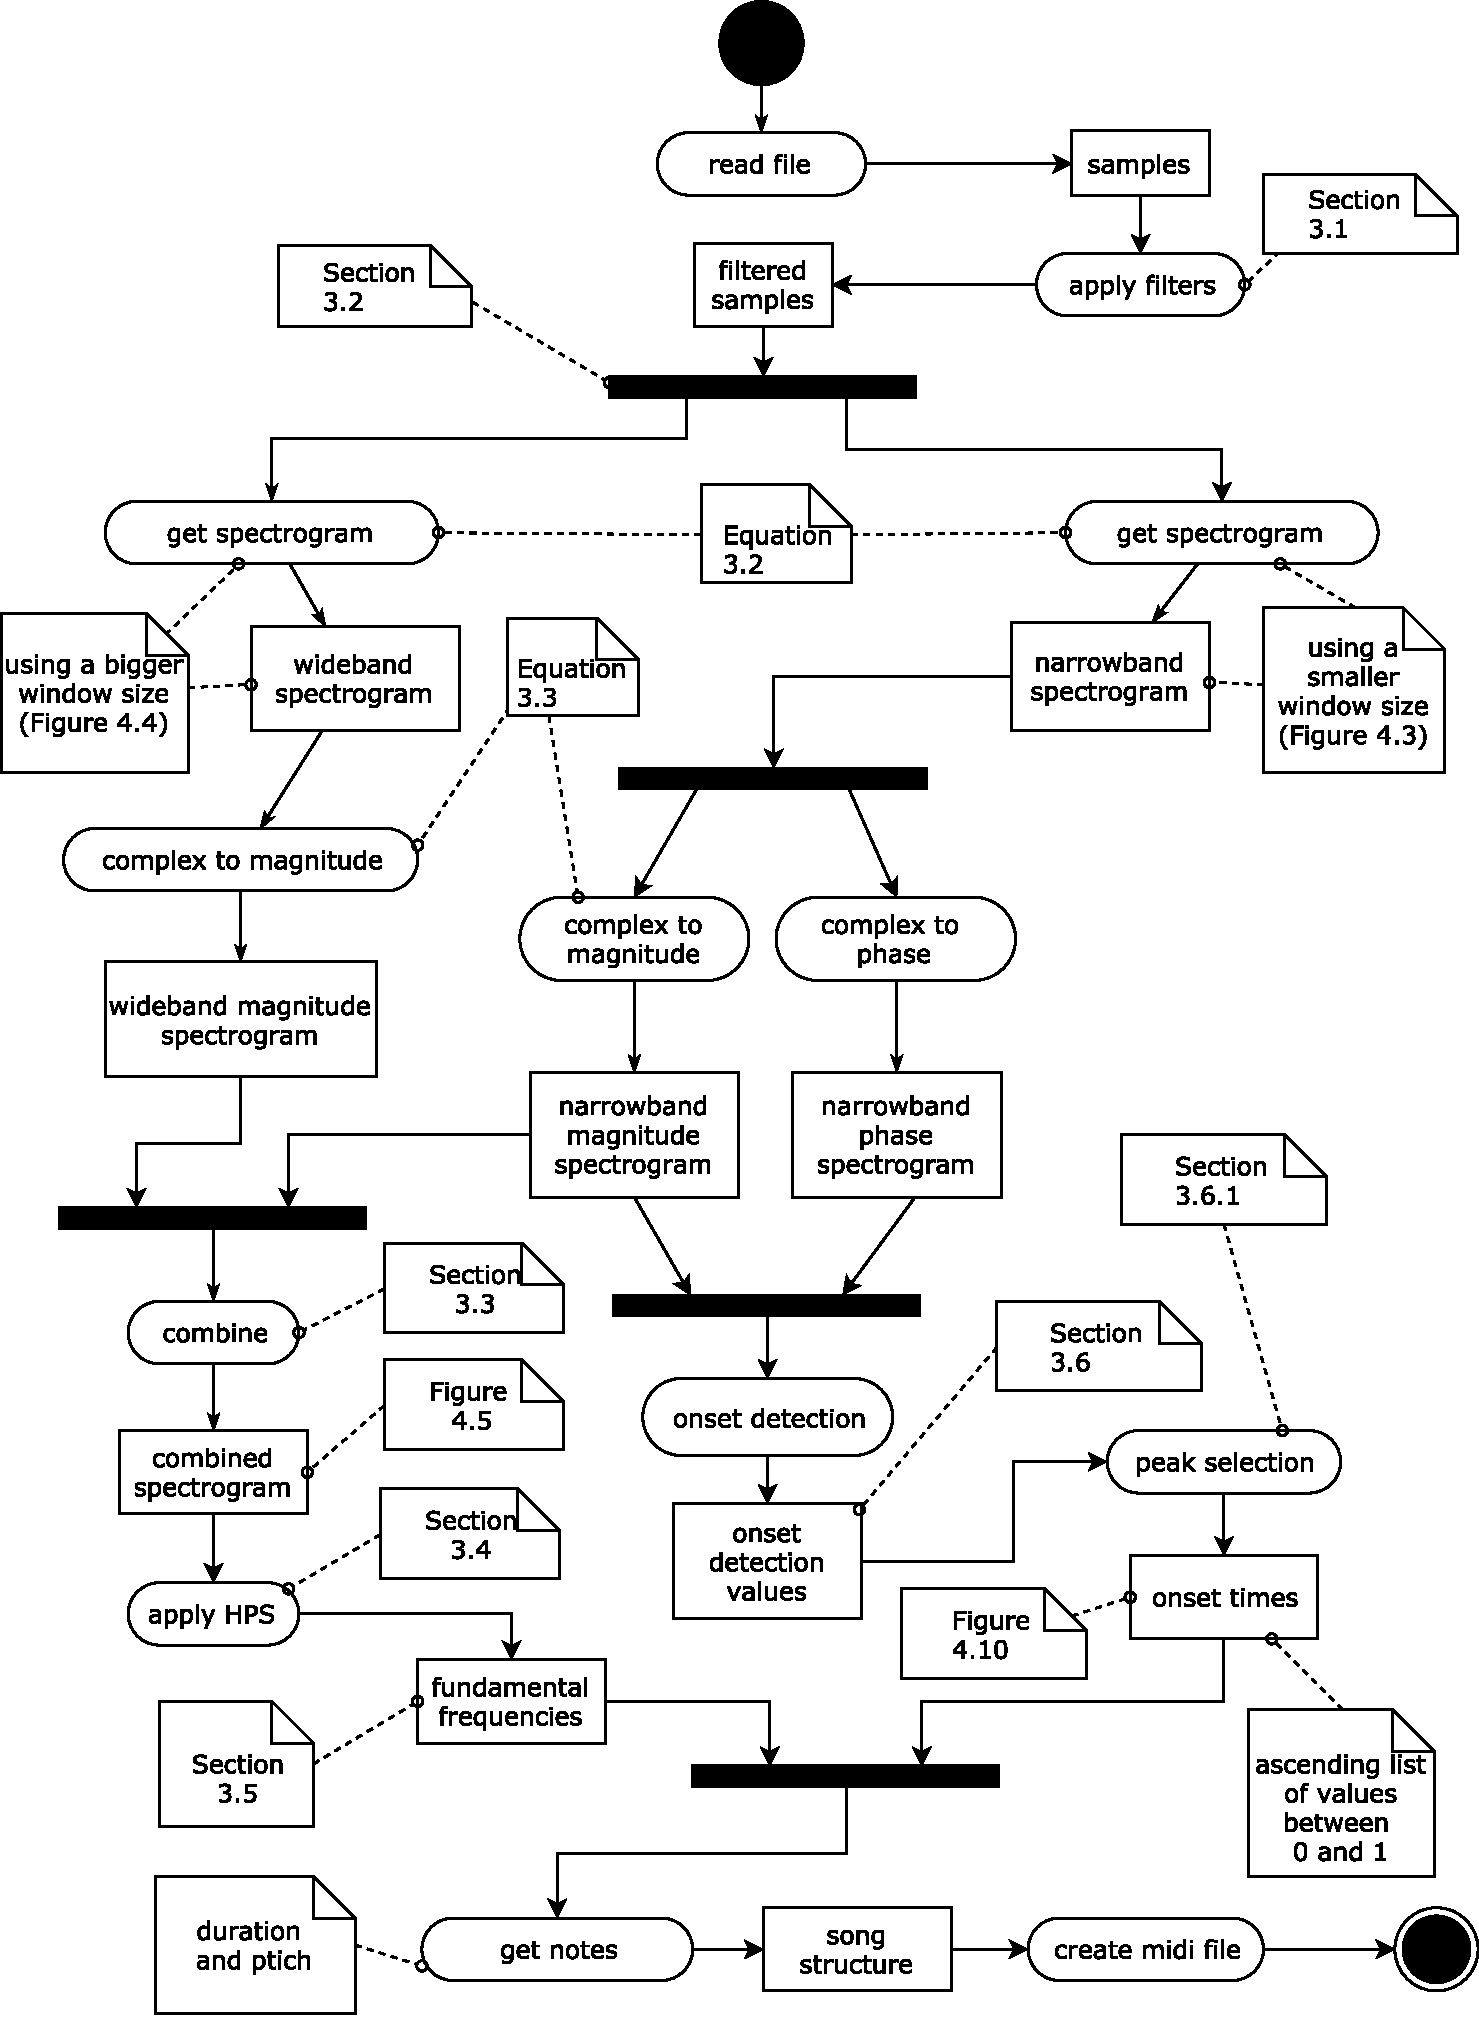
\includegraphics[width=\textwidth,keepaspectratio]{activity.pdf}
\end{center}
\caption{Activity Diagram}
\vskip\baselineskip % Leave a vertical skip below the figure
\label{fig:activity}
\end{figure}

\chapter{DESIGN AND IMPLEMENTATION}
\label{design-and-implementation}
Implementation is written in Rust \cite{rust} for calculation intensive parts while user interface and graphical parts are written in Python. Rust was chosen for its safety for concurrency and speed. Python was chosen for its vast graphics library options. Initially, although calculations were implemented with as much concurrency as possible on the CPU, it still showed to be insufficient in terms of the time it took to finish a complete analysis for relatively long inputs and a reimplementation of the same algorithms on the GPU by utilizing the Arrayfire \cite{arrayfire} library deemed to be necessary. This library uses CUDA framework when possible and falls back to OpenCL or CPU. For simplicity, input files are limited to .wav format. 

Using two different languages required the utilization of foreign function interfaces (FFI) and C style data structures acting as a bridge. Using FFI's prevented any performance hits otherwise would have happened with different approaches such as I/O operations, piping or shared memory. As a design choice Rust source was compiled as a dynamic library and called from Python through its ABI. A graphical interface encapsulates the CLI as an outer layer where the CLI can work by itself by providing all the parameters beforehand. Functions like FFT, resizing, multiplying are called within the Rust code and executed through the backend CUDA Framework during the analysis.

\begin{figure}[htbp]
\begin{center}
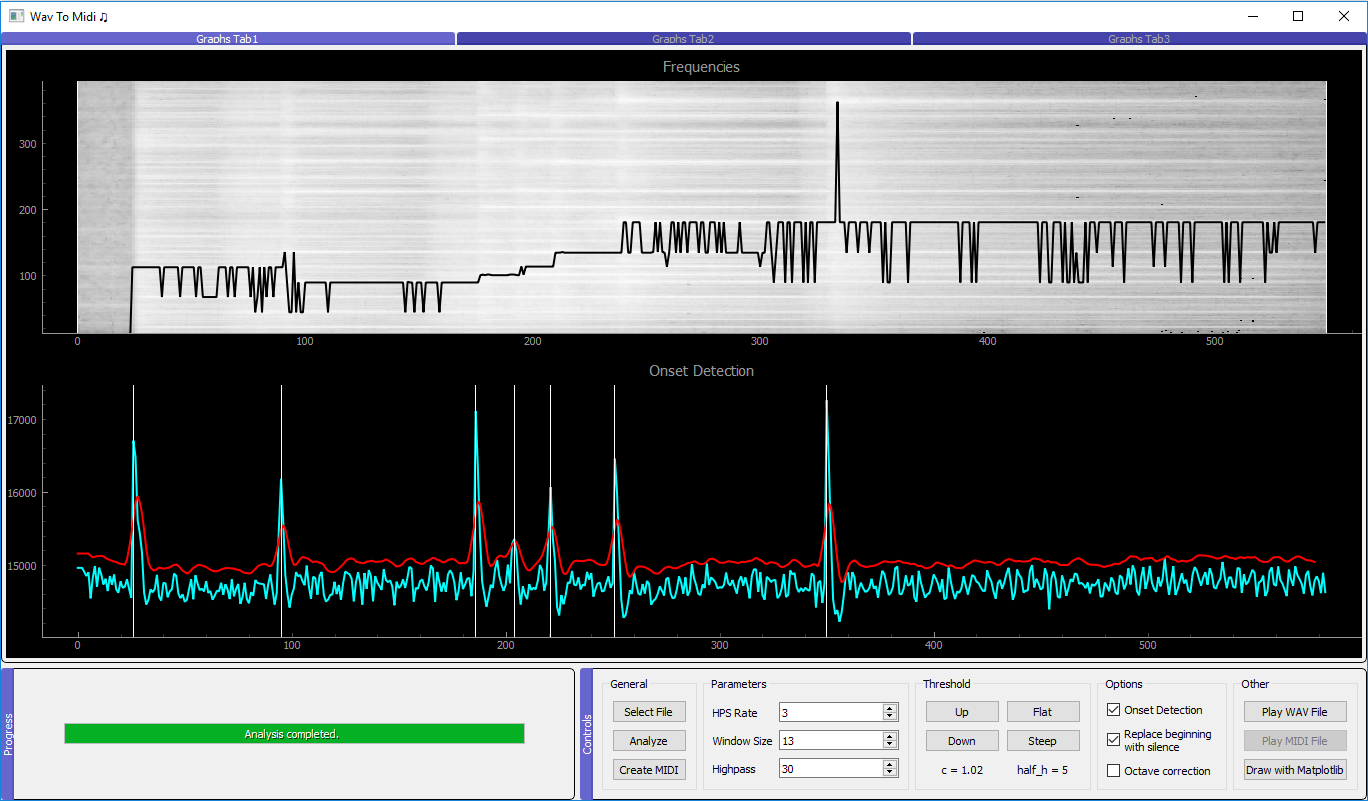
\includegraphics[scale=0.4]{interface.png}
\end{center}
\caption{User Interface}
\vskip\baselineskip 
\label{fig:interface}
\end{figure}
\vskip\baselineskip
\begin{figure}[htbp]
\begin{center}
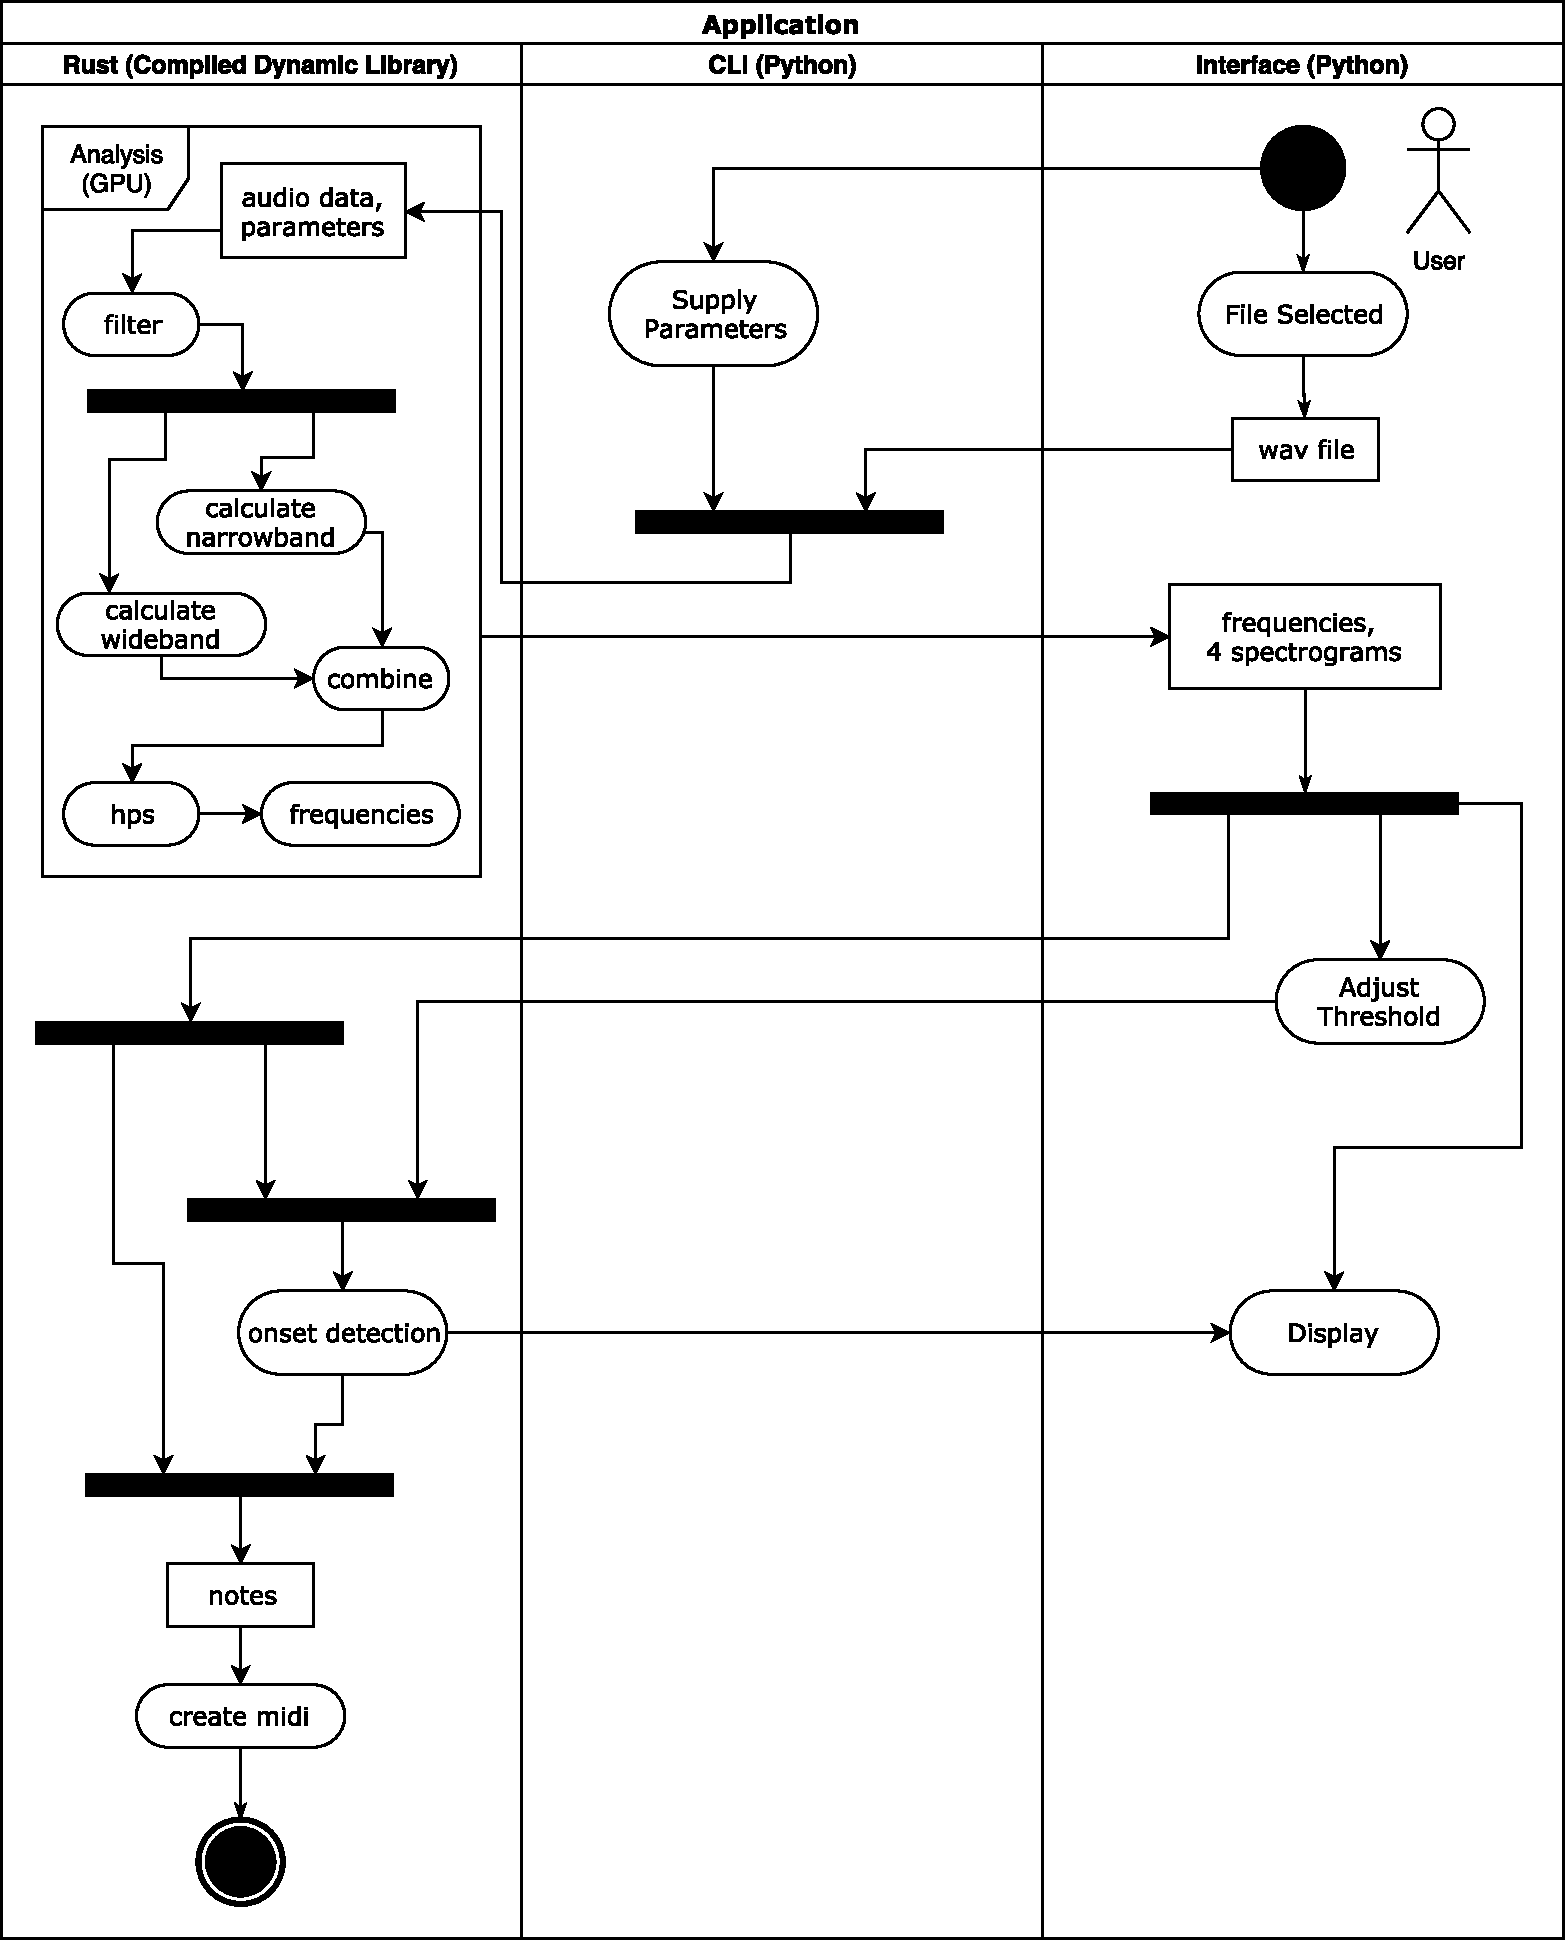
\includegraphics[width=\textwidth,keepaspectratio]{implementation.pdf}
\end{center}
\caption{Implementation Diagram}
\vskip\baselineskip % Leave a vertical skip below the figure
\label{fig:implementation}
\end{figure}

Analysis starts by the user providing the parameters through the interface. If the user does not change the parameters, default values are used which throughout development showed to be generally acceptable but fine tuning of the parameters gives the best results. In the first stage three parameters are required which are the windows size to use in STFT, a highpass frequency for filtering and the HPS rate. HPS rate can be a minimum of 1 which means it will not be applied. A maximum value of 7 is enough as the human hearing spans only 8 octaves. Window size parameter is put as a small integer number $n$ and for the actual window size $2^n$ is used. The reason for using the power of two is that provided FFT algorithms are optimized for such inputs. Step size is set to 1024 for all STFT calculations as it showed to provide sufficient characteristics for both narrowband and wideband spectrograms. Defaults values of the parameters are: 3 for the HPS rate, 13 for window and 30 for the highpass.

It is continued by converting the samples of the audio into an Array structure provided by the ArrayFire library so that the calculations can be continued on the GPU. Second thing is to filter the samples with a convolution function which was also provided within the library. 
After the filtering, two spectrograms are calculated with the user supplied parameters and the filtered samples. Algorithm of the short time Fourier transform with complex valued output is as seen in Figure \ref{alg:stft}

Narrowband spectrogram's windows size comes from the parameter where as wideband spectrogram's is a fixed value of 44100. Wideband spectrogram is used for its characteristics of good frequency resolution and calculating it with a window size of 44100 makes every frequency bin correspond to 1 Hz. The FFT calculations take place in parallel on the GPU to utilize a highly concurrent environment. Narrowband and wideband spectrograms' characteristic properties can be seen in Figure \ref{fig:narrow} and Figure \ref{fig:wide} respectively. Also some frequencies from harmonics are present on some time frames in both figures.

\begin{figure}[htbp]
\begin{center}
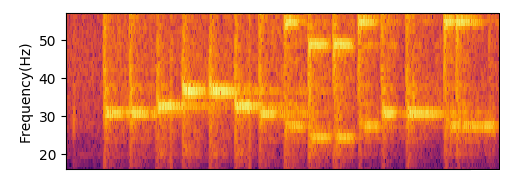
\includegraphics{narrow.png}
\end{center}
\caption{Narrowband Spectrogram}
\vskip\baselineskip % Leave a vertical skip below the figure
\label{fig:narrow}
\end{figure}

A narrowband spectrogram has good time resolution, meaning that note changing points of time are relatively more distinguishable. Therefore it is suitable for the retrieval of information about the onset times and durations of the notes.

\begin{figure}[htbp]
\begin{center}
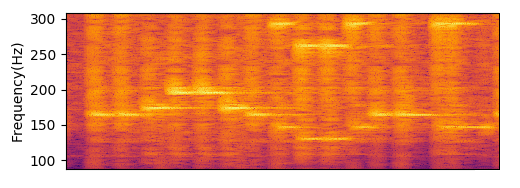
\includegraphics{wide.png}
\end{center}
\caption{Wideband Spectrogram}
\vskip\baselineskip 
\label{fig:wide}
\end{figure}

A wideband spectrogram has good frequency resolution, meaning that the high amplitude frequency bins more accurately represent the actual frequencies. Therefore it is suitable for retrieval of information about the pitch.
\vskip\baselineskip
After both spectrogram calculations are complete they are set to be combined. Combining is done by an element-wise multiplication and requires both to be the same size and shape. For resizing first and multiplying next, provided functions from the ArrayFire library were used as these matrix operations are much faster on the GPU taking advantage of parallelism. Combined spectrogram conveys the characteristic from both which can be seen in Figure \ref{fig:combined}
\vskip\baselineskip
\begin{figure}[htbp]
\begin{center}
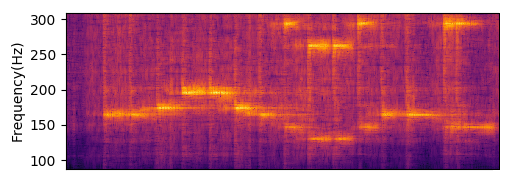
\includegraphics{combined.png}
\end{center}
\caption{Combined Spectrogram}
\vskip\baselineskip
\label{fig:combined}
\end{figure}

Then, using the Equation \ref{eq:hps}, HPS technique is applied to the resulting combined spectrogram. HPS algorithm can be seen in Figure \ref{alg:hps}

HPS applied spectrogram will have the fundamental frequencies standing out with their high amplitudes. The spectrogram can be seen in Figure \ref{fig:hps} with a white line plotting the fundamentals.
\vskip\baselineskip 
\begin{figure}[htbp]
\begin{center}
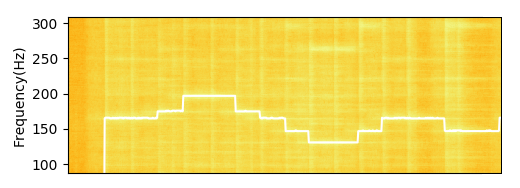
\includegraphics{hps.png}
\end{center}
\caption{HPS Applied Spectrogram}
\vskip\baselineskip 
\label{fig:hps}
\end{figure}
\vskip\baselineskip
Acquiring the fundamentals i.e. the frequencies with the highest amplitude for every time frame is done using the Equation \ref{eq:max-freq} and can be implemented as seen in Figure \ref{alg:freq}

At this point, for some inputs, converting the fundamentals into notes by getting the pitches and durations can be done, such as inputs with no repeating notes and no fluctuations in the fundamentals list. Some violin recordings or computer generated music with few number of harmonics fall into this category. Otherwise the analysis should be continued with the onset detection using the Equation \ref{eq:complex-onset}. On Figure \ref{fig:hps} some visual changes can be observed at places where although the fundamental does not change. These are the repeated notes and will be detected with the onset detection procedure. If the process was started from the graphical user interface, it is now expected from the user to examine and adjust the threshold for onset detection if they wish to do so.

Peak points of the onset detection function which is calculated in Figure \ref{alg:onset} some of which eliminated by the threshold are converted into a value between zero and one where zero is the beginning and one is the end of the audio.
\newpage
Figure \ref{fig:onsets} shows the selected onset times where cyan is the detection function, red is the threshold and the vertical lines are the selected peaks. Between every two onset time is a duration of a note. Number of samples and the length of the audio in seconds is used to calculate a division value for the MIDI file. Division, is a unit delta-time for writing the notes to MIDI. Notes' durations are set in relation to this division value. 
\vskip\baselineskip
\begin{figure}[htbp]
\begin{center}
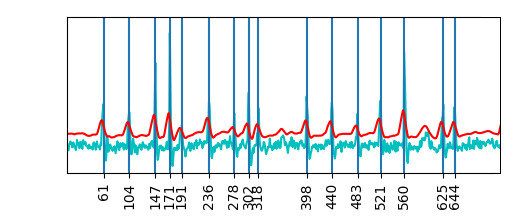
\includegraphics{onsets.png}
\end{center}
\caption{Onsets}
\vskip\baselineskip
\label{fig:onsets}
\end{figure}
\section{GPU Calculations}
Throughout the analysis, ArrayFire's \cite{arrayfire} library functions are used for operations which can benefit from high concurrency. The mainly used operations are: convolution, fft, resizing matrices, interpolation and element-wise operations. The library uses an analogy where host is the CPU and the device is the GPU. Before starting the analysis, samples are put into an internal structure of the library, called \textit{Array}. This data structure can be sent to the device and back through the system BUS and hold in buffers which are internally managed by the library. To minimize the overhead caused by the transfer between the host and the devices and remove it as a bottleneck Array type acts as a pointer, which points to a memory location on the VRAM. To reduce the overhead in the implementation Array data are sent to the device after sampling is done and not transferred back to the host to the very end until no other operations left which can benefit from high concurrency. 

\chapter{TEST AND RESULTS}
\label{test-and-results}
Following test results are acquired from wav files that were converted from MIDI to know the actual notes and have input without noise. MIDI file is a scale run down of D minor pentatonic. Pitch accuracy is calculated by examining time slots and checking whether it matches the original. Whether the octaves are correct or not is not taken into consideration.

\begin{table}[thbp]
\vskip\baselineskip 
\caption[Tests]{Tests.}
\begin{center}
\fontsize{11}{11}\selectfont
\begin{tabular}[width=\textwidth]{|c|c|c|c|c|} \hline 
& Instrument & BPM & Pitch Accuracy & Additional Info \\ \hline 
1 & Guitar  & 100 & \%100 & All notes 1 Octave Below Actual\\ \hline
2 & Piano  & 100 & \%87 & \\ \hline
3 & Violin & 100 & \%83 & Onset Detection off\\ \hline
4 & Guitar  & 150 & \%100 & \\ \hline
5 & Piano  & 150 & \%83 & non-defaults c=1.03,h=5 \\ \hline
6 & Violin  & 150 &\%91  & Onset Detection off\\ \hline
7 & Guitar  & 100* & \%100 & \\ \hline
8 & Piano  & 100* & \%91 & non-defaults HPS:4, c=1.01\\ \hline
9 & Violin  & 100* & \%87 & Onset Detection off\\ \hline
10 & Guitar  & 150* & \%98 & \\ \hline
11 & Piano  & 150* & \%86 & non-defaults c=1.01\\ \hline
12 & Violin  & 150* & \%85 & Onset Detection off\\ \hline
13 & Guitar  & 200* & \%75 & \\ \hline
14 & Piano  & 200* & \%55 & non-defaults c=1.01\\ \hline
15 & Violin  & 200* & \%65 & Onset Detection off\\ \hline
\end{tabular}
\label{table:testing}
\end{center}
*: denoted rows are $16^{th}$, otherwise quarter notes
\end{table}
\vskip\baselineskip
Instruments with low attack rates tend to give better results without onset detection. Results confirmed that the algorithm works better on recordings with definite onsets with high attacks and increasing the note rapidity affects onset detection negatively.
\newpage
Results from speed tests confirmed that reimplementation of the algorithm using GPU showed to be the correct approach regarding processing time. Even though the former utilized all available CPU cores for the calculations, it was not sufficient for moderately long audio inputs and processing times were not acceptable. 
\begin{figure}[htbp]
\begin{center}
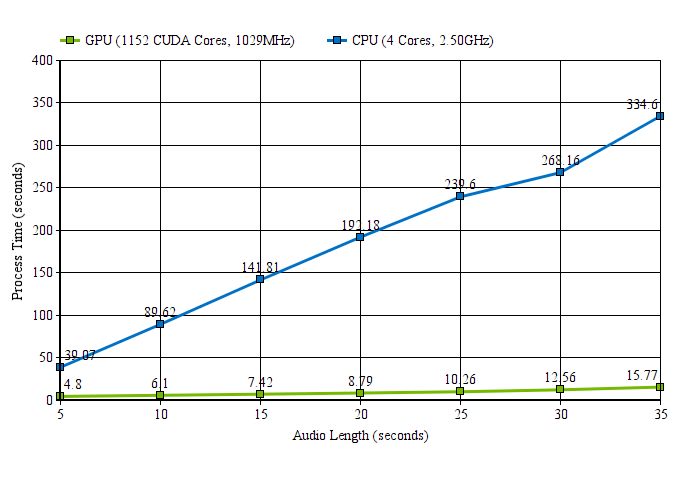
\includegraphics[width=\textwidth]{speed.png}
\end{center}
\caption{Speed Test}
\vskip\baselineskip
\label{fig:speedtest}
\end{figure}

\chapter{CONCLUSION}
\label{chapter:conclusion}

Implemented algorithm has good success rate given that the correct parameters are supplied and a monophonic audio with a high signal to noise ratio is used. Otherwise, improvements are needed.

\section{Future Work}
To improve the algorithm that currently works on monophonic inputs and extend it to work on polyphonic inputs, filter banks can be used by dividing the input into frequency channels and analysing each separately. Current limitation on input audio length infused by the memory of the video card can be solved by dividing the input into time slices and putting them in a queue before applying the same algorithm. Parameters that are currently requested from the user can be automated by implementing decision trees. Also speed tests showed that a real time implementation is possible.

\printbibliography

\appendix
\chapter{RUST CODE}

\fontsize{8}{8}\selectfont
\begin{verbatim}
//lib.rs

#![feature(step_by)]
#![allow(dead_code)]
#![allow(deprecated)]
#![feature(use_extern_macros)]

extern crate hound;
extern crate arrayfire;

use arrayfire::{Array, Dim4, Seq};

use std::f64;
use std::os::raw;
use std::ffi::CString;
use std::path::Path;
use std::slice;

mod spectrogram;
mod filters;
mod postprocess;

#[repr(C)]
pub struct FFI_Spectrogram {
    data : *const *const raw::c_double,
    shape : (u64, u64),
}

#[no_mangle]
pub fn analyze(file_name: *const raw::c_char, window_size: raw::c_uint, highpass: raw::c_uint, 
               hps_rate: raw::c_uint) -> *const *const raw::c_void
{
    //println!("Active Backend: {}", arrayfire::get_active_backend());
    
    println!("reading file...");
    let name: String = unsafe{std::ffi::CStr::from_ptr(file_name)}.to_string_lossy().into_owned();
    let mut reader = hound::WavReader::open(name.clone()).unwrap();

    //print_audio_details(&reader);

    let data : Vec<f64> = reader.samples::<i16>().map(|sample| sample.unwrap() as f64).collect();
    let mut data_af = Array::new(&data, Dim4::new(&[data.len() as u64,1,1,1])); 
  
    println!("applying preprocess filters..."); // TODO: filters as parameters
    data_af = ::filters::highpass(data_af, highpass as usize);
    //data_af = ::filters::lowpass(data_af, 330);

    let mut graphs = Vec::<*const raw::c_void>::new();        

    println!("calculating narrowband spectrogram...");
    let window_size = (2. as f64).powi(window_size as i32) as usize;
    let complex = spectrogram::stft(&data_af, window_size, 1024);
    let narrowband = spectrogram::complex_to_magnitude(&complex);
    graphs.push(to_ffi(&spectrogram::to_host(&narrowband)));
    
    println!("calculating wideband spectrogram...");
    let wideband = spectrogram::get_spectrogram(&data_af, 44100, 1024);
    graphs.push(to_ffi(&spectrogram::to_host(&wideband)));

    println!("combining spectrograms...");
    let combined = spectrogram::combine(&narrowband, &wideband);
    graphs.push(to_ffi(&spectrogram::to_host(&combined)));    

    println!("calculating harmonic product spectrum...");
    let hps = spectrogram::harmonic_product_spectrum(combined, hps_rate);
    graphs.push(to_ffi(&spectrogram::to_host(&hps)));    

    println!("getting frequencies...");
    let frequencies = spectrogram::get_frequencies(&hps);
    let mut frequencies_host : Vec<raw::c_uint> = vec![0; frequencies.elements()];
    frequencies.host(frequencies_host.as_mut_slice());
    let freq_p = Box::into_raw(frequencies_host.into_boxed_slice()) as *const raw::c_uint;
    graphs.push(freq_p as *const raw::c_void);

    println!("onset detection function...");
    let phase = spectrogram::complex_to_phase(&complex);
    let complex_df = spectrogram::onset_detection(&narrowband, &phase);
    let detect_p = Box::into_raw(complex_df.into_boxed_slice()) as *const raw::c_double;
    graphs.push(detect_p as *const raw::c_void);

    println!("Analysis completed.");    
    arrayfire::device_gc();

    Box::into_raw(graphs.into_boxed_slice()) as *const *const raw::c_void
}

fn to_ffi(s : &Vec<Vec<f64>>) -> *const raw::c_void
{
    let p_array : Vec<*const raw::c_double> = 
        s.iter().map(|c| Box::into_raw(c.clone().into_boxed_slice()) as *const raw::c_double).collect();
        
    let spect = FFI_Spectrogram {
        shape : (s.len() as u64, s[0].len() as u64),
        data : Box::into_raw(p_array.into_boxed_slice()) as *const *const raw::c_double
    };

    Box::into_raw(Box::new(spect)) as *const raw::c_void
}

fn post_filter(spectrogram: &Array, above: usize, below: usize) -> Array
{
    let sequence0 = Seq::new(above as u32, below as u32, 1);
    let sequence1 = Seq::new(0, (spectrogram.dims()[1]-1) as u32, 1);
    let mut idxr = arrayfire::Indexer::new();            
    idxr.set_index(&sequence0, 0, Some(true));
    idxr.set_index(&sequence1, 1, Some(true));    
  
    arrayfire::index_gen(&spectrogram, idxr)
}

#[no_mangle]
pub extern fn clean2d( ptr : *const raw::c_void) 
{
    unsafe 
    { 
        let ffi_spect = Box::from_raw(ptr as *mut FFI_Spectrogram);
        let data = std::slice::from_raw_parts(ffi_spect.data, ffi_spect.shape.0 as usize);
        for x in 0..data.len() { Box::from_raw(data[x] as *mut f64); }
    }
}

#[no_mangle]
pub extern fn clean1d( ptr : *const raw::c_void)
{
    unsafe { Box::from_raw(ptr as *mut raw::c_double) };
}

fn print_audio_details(reader: &hound::WavReader<std::io::BufReader<std::fs::File>>) 
{
    print!("Audio: {{ Duration: {} seconds, ", reader.duration() / reader.spec().sample_rate);
    print!("Sample Rate: {}, ", reader.spec().sample_rate);
    print!("Channels: {}, ", reader.spec().channels);
    println!("Bit Depth: {} }}", reader.spec().bits_per_sample);
}

#[no_mangle]
pub extern fn create_midi(frequencies: *mut raw::c_uint, f_len: raw::c_uint,
                           onsets: *mut raw::c_double, o_len: raw::c_uint, 
                           file_name: *const raw::c_char, onset_detection: bool) -> *const raw::c_char
{
    let name: String = unsafe { std::ffi::CStr::from_ptr(file_name).to_string_lossy().into_owned() };
    let reader = hound::WavReader::open(&name).unwrap();
    
    // division = 1 beat = 1 seconds
    let seconds = reader.duration() as f64 / reader.spec().sample_rate as f64;
    let division : i16 = (f_len as f64 / seconds) as i16;

    let f : &[u32] = unsafe { slice::from_raw_parts(frequencies, f_len as usize) };
    let o : &[f64] = unsafe { slice::from_raw_parts(onsets, o_len as usize) };    

    let notes = postprocess::get_notes(&f.to_vec(), &o.to_vec(), onset_detection);
    
    let midi_name = String::from(Path::new(name.as_str()).file_stem().unwrap().to_str().unwrap());
    let song = postprocess::Song {notes: notes, name: midi_name, division: division};

    //println!("{}", song);
    let midi_filename = postprocess::write_midi(song);
    println!("writing to {}.mid", midi_filename);
    CString::new(midi_filename).unwrap().into_raw()
}
\end{verbatim}
\newpage
\begin{verbatim}
//spectrogram.rs

extern crate apodize;

use arrayfire::*;
use self::apodize::{hanning_iter};
use std::f64;

type Column = Vec<f64>;
type Spectrogram = Vec<Column>;

pub fn get_spectrogram(audio_data : &Array, window_size: usize, step_size: usize) -> Array
{
    let array = stft(audio_data, window_size, step_size);
    complex_to_magnitude(&array)
}

pub fn complex_to_magnitude(stft: &Array) -> Array
{
    let spect_len = stft.dims()[1];
    let result = Array::new_empty(stft.dims(), DType::F64);

    for index in 0..spect_len
    {
        set_col(&result, &magnitude(&col(&stft, index)), index);
    }

    return result;
}

pub fn complex_to_phase(stft: &Array) -> Array
{
    let spect_len = stft.dims()[1];
    let result = Array::new_empty(stft.dims(), DType::F64);    

    for index in 0..spect_len
    {
        set_col(&result, &phase(&col(&stft, index)), index);
    }

    return result;
}

pub fn stft(audio_data : &Array, window_size: usize, step_size: usize) -> Array
{
    let audio_len : usize = audio_data.elements();

    let spect_len : u64 = (( audio_len-(window_size-step_size) ) / step_size) as u64;
    let array = Array::new_empty(Dim4::new(&[window_size as u64, spect_len, 1,1]), DType::C64);

    let hanning_len = Dim4::new(&[window_size as u64,1,1,1]);
    let hanning = Array::new(&hanning_iter(window_size as usize).collect::<Vec<f64>>(), hanning_len);

    for (index, start) in (0..audio_len-window_size).step_by(step_size).enumerate()
    {
        let sequence =  Seq::new(start as u32, start as u32 + (window_size-1) as u32, 1);
        let mut idxr = Indexer::new();                
        idxr.set_index(&sequence, 0, Some(true));

        let new_col = fft(&(index_gen(&audio_data, idxr) * hanning.clone()), 1., window_size as i64);
        set_col(&array, &new_col, index as u64); 
    }

    return get_half(&array);
}

fn get_half(stft: &Array) -> Array
{
    let sequence0 = Seq::new(0, ((stft.dims()[0] as f32 / 2.).floor()-1.) as u32, 1);
    let sequence1 = Seq::new(0, (stft.dims()[1]-1) as u32, 1);    
    let mut idxr = Indexer::new();            
    idxr.set_index(&sequence0, 0, Some(true));
    idxr.set_index(&sequence1, 1, Some(true));    
    
    index_gen(&stft, idxr)
}

fn magnitude(col : &Array) -> Array
{
    let magnitude = sqrt( &(pow(&real(&col),&2, true) * pow(&imag(&col),&2, true)) );
    floor(&log1p(&magnitude))
}

fn phase(col: &Array) -> Array
{
    atan2(&imag(col), &real(col), true)
}

pub fn onset_detection(m: &Array, p: &Array) -> Vec<f64>
{
    let mut result : Vec<f64> = Vec::new();

    let spect_len = m.dims()[1];
    for index in 2..spect_len
    {
        let predicted_m = col(&m, index-1);
        let predicted_p = mul(&col(&p, index-1),&2, true) - col(&p, index-2);

        let a = col(&m, index) - predicted_m;
        let rectified = (&a + abs(&a))/2;
        let b = col(&p, index) - predicted_p;
        let distance = sqrt(&(pow(&rectified, &2, true) + pow(&b, &2, true))); 

        result.push(sum_all(&distance).0);
    }

    let mut v = vec![result[0];2];
    v.extend(result);
    return v;
}

pub fn combine(narrowband : &Array, wideband : &Array) -> Array
{
    let wd = wideband.dims();
    let narrow = resize(&narrowband, wd[0] as i64, wd[1] as i64, InterpType::BILINEAR);
    mul(wideband, &narrow, true)
}

pub fn harmonic_product_spectrum(combined : Array, rate : u32) -> Array
{
    let sequence0 = Seq::new(0 as u32, ((combined.dims()[0] as f32 / rate as f32)-1.) as u32, 1);
    let sequence1 = Seq::new(0 as u32, (combined.dims()[1]-1) as u32, 1);
    let mut idxr = Indexer::new();            
    idxr.set_index(&sequence0, 0, Some(true));
    idxr.set_index(&sequence1, 1, Some(true));    
  
    let mut hps = index_gen(&combined, idxr);

    for r in 2..rate+1
    {
        let scale = (combined.dims()[0] as f32 / r as f32) as i64;
        let downsampled = resize(&combined, scale, combined.dims()[1] as i64, InterpType::BILINEAR);

        let mut idxr = Indexer::new();            
        idxr.set_index(&sequence0, 0, Some(true));
        idxr.set_index(&sequence1, 1, Some(true)); 
        hps *= index_gen(&downsampled, idxr);
    }

    return log1p(&hps);
}

pub fn get_frequencies(spectrogram: &Array) -> Array
{
    imax(&spectrogram, 0).1
}

pub fn to_host(spectrogram_af : &Array) -> Spectrogram
{
    let window_size = spectrogram_af.dims()[0];
    let slice_len = window_size * spectrogram_af.dims()[1];
    let mut host = vec![0.; slice_len as usize];
    spectrogram_af.host::<f64>(host.as_mut_slice());

    let mut spectrogram : Spectrogram = Vec::new();
    for column in host.chunks(window_size as usize)
    {
        spectrogram.push(column.to_vec());
    }

    return spectrogram;
}
\end{verbatim}
\newpage
\begin{verbatim}
//postprocess.rs

extern crate rimd;

use std::{f64, fmt};
use self::rimd::{ TrackEvent, Event, MidiMessage, SMFWriter, SMFFormat, Track, SMF};
use std::path::Path;
use std::collections::HashMap;

pub struct Note {name: String, midi: u8, duration: u64}
pub struct Song{pub notes: Vec<Note>, pub division: i16, pub name: String}

impl fmt::Display for Song {
    fn fmt(&self, f: &mut fmt::Formatter) -> fmt::Result {
        let all_notes : String = 
            self.notes.iter().fold(String::new(), |s, n| 
                format!("{}{}", s, format!("{}[{}] ", n.name, n.duration)));
        write!(f, "{}: {}", self.name, all_notes)
    }
}

fn get_pitch(frequency : u32) -> (String, u8) 
{
    if frequency < 16 { return (String::from("R"), 0); }

    let notes = vec![ "C", "C#/Db", "D", "D#/Eb", "E", "F", "F#/Gb", "G", "G#/Ab", "A", "A#/Bb", "B" ];
    
    //distance to A440 of the note
    let log_base : f64 = (2.0 as f64).powf(1.0/12.0);   
    let mut offset : i32 = ((frequency as f64 / 440.0).log(log_base)).round() as i32;

    let midi = 69 + offset; // A4 in midi is 69
    
    //adjust offset for the array
    offset += if offset >= 0 {9} else {-2}; 
    let note_index : usize = if offset >= 0 {offset%12} else {11 + offset%12} as usize;
    return (format!( "{note}{octave}", note = notes[note_index], octave = 4 + offset/12), midi as u8);
}

pub fn get_notes(frequencies: &[u32], onsets: &[f64], no_onset: bool) -> Vec<Note>
{
    let vec : Vec<(String, u8)> = frequencies.iter().map(|freq| get_pitch(*freq)).collect();
    let mut notes : Vec<Note> = Vec::new();

    if no_onset
    {
        let mut last: usize = 0;
        for i in 1..vec.len()
        {
            if vec[i] != vec[i-1] || i == vec.len()-1 {
                notes.push( Note { 
                    name: vec[i-1].0.clone(), midi: vec[i-1].1.clone(), 
                    duration: (i-last) as u64 
                } );
                last = i;
            }
        }
    }
    else
    {
        let mut onsets_clone : Vec<f64> = onsets.clone().to_vec();
        onsets_clone.push(1.);
        let mut previous_onset : f64 = 0.;
        for &onset in &onsets_clone
        {
            let start_index : usize = (frequencies.len() as f64 * previous_onset).round() as usize;
            let end_index : usize = (frequencies.len() as f64 * onset).round() as usize;

            let interval : &[(String,u8)] = &vec[start_index..end_index];

            let mode = mode(interval);
            let duration : u64 = end_index as u64 - start_index as u64;

            notes.push( Note {
                name: mode.0.clone(), midi: mode.1.clone(),  duration: duration
            });

            previous_onset = onset;
        }
    }


    return notes;
}

fn mode(elements: &[(String,u8)]) -> &(String,u8) {

    let mut occurrences = HashMap::new();

    for value in elements {
        *occurrences.entry(value).or_insert(0) += 1;
    }

    occurrences.into_iter()
        .max_by_key(|&(_, count)| count)
        .map(|(val, _)| val)
        .expect("Cannot compute the mode of zero elements")
}

pub fn write_midi(song: Song) -> String
{   
    let mut midi_filename = song.name.clone();
    let mut events : Vec<TrackEvent> = Vec::new();

    let mut previous_duration = 0;
    for note in song.notes.iter() 
    {
        if note.name != "R" 
        {
            events.push( TrackEvent { 
                event: Event::Midi(MidiMessage::note_on(note.midi, 125, 0)), 
                vtime: previous_duration
            } );
        
            events.push( TrackEvent { 
                event: Event::Midi(MidiMessage::note_off(note.midi, 125, 0)), 
                vtime: note.duration 
            } );
        }

        if note.name == "R" { 
            previous_duration += note.duration;
        } else {
            previous_duration = note.duration as u64;
        }

    }

    let tracks = vec![ Track {copyright: None, name: None, events: events} ];
    let smf = SMF {format: SMFFormat::Single, tracks: tracks, division: song.division};
    let writer = SMFWriter::from_smf(smf);
 
    let result = writer.write_to_file(Path::new(format!("{}{}", song.name,".mid").as_str()));
    if result.is_err()
    {
        let song_ = Song {notes: song.notes, name: song.name+"_", division: song.division};
        midi_filename = write_midi(song_);
    }

    return midi_filename;
}

//filters.rs

extern crate synthrs;
use self::synthrs::filter::{cutoff_from_frequency, highpass_filter, lowpass_filter};
use arrayfire::{Array, Dim4, convolve1, ConvMode, ConvDomain};

pub fn highpass(signal: Array, h: usize) -> Array
{
    let highpass = highpass_filter(cutoff_from_frequency(h as f64, 44100), 0.01); 
    let filter : Array = Array::new(&highpass, Dim4::new(&[highpass.len() as u64,1,1,1]));
    convolve1(&signal, &filter, ConvMode::DEFAULT, ConvDomain::FREQUENCY)
}

pub fn lowpass(signal: Array, l: usize) -> Array
{
    let lowpass = lowpass_filter(cutoff_from_frequency(l as f64, 44100), 0.01);
    let filter : Array = Array::new(&lowpass, Dim4::new(&[lowpass.len() as u64,1,1,1]));
    convolve1(&signal, &filter, ConvMode::DEFAULT, ConvDomain::FREQUENCY)
}
\end{verbatim}
\newpage
\begin{verbatim}
# Cargo.toml

[package]
name = "rust_test"
version = "0.1.0"
authors = ["utku <utkuce@gmail.com>"]

[lib]
name = "mylib"
crate-type = ["dylib"]

[dependencies]
hound = "3.1.0" # read wav file
rimd = "0.0.1" # midi
arrayfire = "3.5.0" # gpu acceleration
apodize = "*" # windowing function

[dependencies.synthrs]
git = "https://github.com/gyng/synthrs" # filters
\end{verbatim}

\chapter{PYTHON CODE}
\begin{verbatim}
#analyze.py

from ctypes import cdll, c_void_p, c_double, c_uint, cast
import argparse
import time
import internal_utility as iu

parser = argparse.ArgumentParser(description='Converts a monophonic wav file into MIDI')

parser.add_argument('-f', '--file-name',
    help='The file that is to be analyzed',
    required=True, type=str)

parser.add_argument('-w','--window', 
    help='2 raised to the w will be used as window length for narrowband spectrogram', 
    required=False, default=13, type=int)

parser.add_argument('-p', '--highpass', 
    help='highpass filter frequency for preprocessing',
    required=False, default=30, type=int)

parser.add_argument('-r', '--hps-rate', 
    help='the rate used for harmonic product spectrum',
    required=False, default=3, type=int)

parser.add_argument('-o', '--onset-window',
    help='half the length of the sliding window used for onset detection thresholding',
    required=False, default=5, type=int)

parser.add_argument('-c', '--threshold-constant',
    help='constant value for scaling the threshold for onset detection',
    required=False, default=1.05, type=float)

parser.add_argument('-i', '--from-interface',
    help='flag to determine if the script is called from the interface',
    action='store_true')

parser.add_argument('-n', '--no-onsets',
    help='flag to use onset detection or not', action='store_true')

args = vars(parser.parse_args())

start_time = time.time()

mylib = cdll.LoadLibrary('target\debug\mylib.dll')
mylib.analyze.restype = c_void_p

results = mylib.analyze(args['file_name'].encode('UTF-8'), args['window'], 
                        args['highpass'], args['hps_rate'])

graphs = iu.from_ffi(results)  


if not args['from_interface']:

    (frequencies, detection) = (graphs[4],  graphs[5])

    (peaks, threshold) = iu.peaks(detection, args['onset_window'], args['threshold_constant'])
    onsets = [ i / len(detection) for i in peaks ]

    print("Finished in %s seconds" % int(time.time() - start_time))    

    mylib.create_midi((c_uint * len(frequencies))(*frequencies), len(frequencies),
                    (c_double * len(onsets))(*onsets), len(onsets),
                    args['file_name'].encode('UTF-8'), args['no_onsets'])

    print("Finished in %s seconds" % (time.time() - start_time))
    exec(open('spectrogram.py').read(), globals(), locals())

else:

    import pickle
    with open('results.temp', 'wb') as f:
        pickle.dump( graphs, f )

mylib.clean2d.argtypes = [c_void_p]
mylib.clean1d.argtypes = [c_void_p]

for i,g in enumerate(iu.pointerList.pointers):
    ptr = cast(g, c_void_p)
    mylib.clean2d(ptr) if i < 4 else mylib.clean1d(ptr)     
\end{verbatim}

\begin{verbatim}
# internal_utility.py

from __future__ import division
import numpy as np
from ctypes import *

class C_Tuple(Structure):
    _fields_ = [("x", c_uint64), ("y", c_uint64)]

class FFI_Spectrogram(Structure):
    _fields_ = [("data", POINTER(POINTER(c_double))), ("shape", C_Tuple)]

class PointerList(Structure):
    _fields_ = [("pointers", c_void_p*6)]

pointerList = PointerList()

def from_ffi(results):
    
    global pointerList
    pointerList = cast(results, POINTER(PointerList)).contents

    spect_list = []

    for i,g in enumerate(pointerList.pointers):
        if i < 4:
            spect_list.append(get_result(g))
        elif i == 4:
            pointer = cast(g, POINTER(c_uint*len(spect_list[3])))
            spect_list.append(np.fromiter(pointer.contents, dtype=np.uint))
        else:
            pointer = cast(g, POINTER(c_double*(len(spect_list[0]-1)) ))
            spect_list.append(np.fromiter(pointer.contents, dtype=float))
        
    return spect_list

def get_result(spect_pointer):

    result = cast(spect_pointer, POINTER(FFI_Spectrogram)).contents

    data = []

    for x in range(0, result.shape.x):
        array_pointer = cast(result.data[x], POINTER(c_double*result.shape.y))
        a = np.frombuffer(array_pointer.contents, dtype=float)
        data.append(a)
    
    return np.asarray(data)

def maximas(data):

    derivative = np.diff(data)
    maximas = []

    for i in range(1, len(data)-1):
        if data[i] - data[i-1] > 0 and data[i] - data[i+1] > 0:
            maximas.append(i)

    return maximas

def peaks(onset, half_h, c1):

    peaks = []
    maximas_indices = maximas(onset)
    dynamic_threshold = []

    for i in range(half_h, len(onset)-half_h):
        window = onset[i-half_h: i+half_h-1]
        weights = list(range(1,half_h,1)) + list(range(half_h,0,-1))
        dynamic_threshold.append(c1*np.average(window, weights=weights))

    for i in range(5):
        dynamic_threshold.insert(0, dynamic_threshold[0])
    
    i = 0
    while i < len(dynamic_threshold) and i < len(onset):
        if onset[i] > dynamic_threshold[i] and i in maximas_indices:
            if set(range(i-half_h, i+half_h)).isdisjoint(peaks):
                peaks.append(i)
            else:
                for (j,p) in enumerate(peaks):
                    if p in list(range(i-half_h, i+half_h)) and onset[i]>onset[p]:
                        peaks[j] = i
        i+=1    

    return (peaks, dynamic_threshold)

def repeated_notes(peaks, changes, half_h, index_scale):

    repeats = []
    for p in peaks:
        l = range(round((p-half_h)*index_scale), round((p+half_h)*index_scale),1)
        if set(l).isdisjoint(changes):
            repeats.append(p)

    return repeats

def octave_correction(frequencies, wideband):

    corrected = []
    for (index,f) in enumerate(frequencies):

        if f == 0:
            corrected.append(0)
            continue

        i = 2
        current_max = f
        while f*i < wideband.shape[1]/2:
            if wideband[index][f*i] > wideband[index][current_max]:
                current_max = f*i
            i += 1

        corrected.append(current_max)

    return corrected
\end{verbatim}

\end{document}
